\documentclass{article}

\usepackage{fancyhdr}
\usepackage{extramarks}
\usepackage{amsmath}
\usepackage{amsthm}
\usepackage{amsfonts,bm}
\usepackage{tikz}
\usepackage[plain]{algorithm}
\usepackage{algpseudocode}
\usepackage{enumerate}
\usepackage{epstopdf}
\usepackage{caption}
\usepackage{graphicx}
\usetikzlibrary{automata,positioning}

%
% Basic Document Settings
%

\topmargin=-0.45in
\evensidemargin=0in
\oddsidemargin=0in
\textwidth=6.5in
\textheight=9.0in
\headsep=0.25in

\linespread{1.1}

\pagestyle{fancy}
%\lhead{\hmwkAuthorName}
%\chead{\hmwkClass\ (\hmwkClassInstructor): \hmwkTitle\ Solutions}
\rhead{}
%\lfoot{\lastxmark}
%\cfoot{\thepage}

\renewcommand\headrulewidth{0.4pt}
\renewcommand\footrulewidth{0.4pt}

\setlength\parindent{0pt}

%
% Create Problem Sections
%

\newcommand{\enterProblemHeader}[1]{
    \nobreak\extramarks{}{Problem \arabic{#1} continued on next page\ldots}\nobreak{}
    \nobreak\extramarks{Problem \arabic{#1} (continued)}{Problem \arabic{#1} continued on next page\ldots}\nobreak{}
}

\newcommand{\exitProblemHeader}[1]{
    \nobreak\extramarks{Problem \arabic{#1} (continued)}{Problem \arabic{#1} continued on next page\ldots}\nobreak{}
    \stepcounter{#1}
    \nobreak\extramarks{Problem \arabic{#1}}{}\nobreak{}
}

\setcounter{secnumdepth}{0}
\newcounter{partCounter}
\newcounter{homeworkProblemCounter}
%\setcounter{homeworkProblemCounter}{1}
%\nobreak\extramarks{Problem \arabic{homeworkProblemCounter}}{}\nobreak{}

%
% Homework Problem Environment
%
% This environment takes an optional argument. When given, it will adjust the
% problem counter. This is useful for when the problems given for your
% assignment aren't sequential. See the last 3 problems of this template for an
% example.
%
\newenvironment{homeworkProblem}[1][-1]{
    \ifnum#1>0
        \setcounter{homeworkProblemCounter}{#1}
    \fi
    \section{Problem \arabic{homeworkProblemCounter}}
    \setcounter{partCounter}{1}
    \enterProblemHeader{homeworkProblemCounter}
}{
    \exitProblemHeader{homeworkProblemCounter}
}

%
% Homework Details
%   - Title
%   - Due date
%   - Class
%   - Section/Time
%   - Instructor
%   - Author
%

\newcommand{\hmwkTitle}{Homework\ \#10}
\newcommand{\hmwkDueDate}{December 4, 2022}
\newcommand{\hmwkClass}{Probability and Statistics for EECS}
%\newcommand{\hmwkClassTime}{Lecture 1}
\newcommand{\hmwkClassInstructor}{Professor Ziyu Shao}
%\newcommand{\hmwkAuthorName}{Ming Li}

%
% Title Page
%

\title{
    \vspace{2in}
    \textmd{\textbf{\hmwkClass:\\ \hmwkTitle}}
    \textmd{\textbf{Solutions}}\\
    \vspace{0.1in}\large{\textit{\hmwkClassInstructor}}
    \vspace{3in}
}

%\author{\textbf{\hmwkAuthorName}}
\date{}

\renewcommand{\part}[1]{\textbf{\large Part \Alph{partCounter}}\stepcounter{partCounter}\\}

%
% Various Helper Commands
%

% Useful for algorithms
\newcommand{\alg}[1]{\textsc{\bfseries \footnotesize #1}}

% For derivatives
\newcommand{\deriv}[1]{\frac{\mathrm{d}}{\mathrm{d}x} (#1)}

% For partial derivatives
\newcommand{\pderiv}[2]{\frac{\partial}{\partial #1} (#2)}

% Integral dx
\newcommand{\dx}{\mathrm{d}x}

% Alias for the Solution section header
\newcommand{\solution}{\textbf{\large Solution}}

% Probability commands: Expectation, Variance, Covariance, Bias
\newcommand{\E}{\mathrm{E}}
\newcommand{\Var}{\mathrm{Var}}
\newcommand{\Cov}{\mathrm{Cov}}
\newcommand{\Bias}{\mathrm{Bias}}


\begin{document}

\maketitle

\pagebreak

\begin{homeworkProblem}[1]

Let $U_i \sim \operatorname{Unif}(0,1), i \geq 1$ be i.i.d. random variables. Define $N$ as follows:
$$
N=\max \left\{n: \prod_{i=1}^n U_i \geq e^{-1} \cdot\right\}
$$
\begin{enumerate}[(a)]
\item Estimate $\mathrm{E}(N)$ by generating 5000 values of $N$ and then use the sample mean.
\item Estimate $\operatorname{Var}(N)$.
\item Estimate $P(N=i)$, for $i=0,1,2,3$.
\item Can you find the exact distribution of $N$ ?
\end{enumerate}

\solution

See the code file.

\end{homeworkProblem}

\pagebreak

\begin{homeworkProblem}[2]

\begin{enumerate}[(a)]
	\item Use the following transformation to generate samples from bivariate Normal distribution with correlation coefficient $\rho$:
	\begin{equation*}
	\begin{aligned}
		& X = Z \\
		& Y = \rho Z + \sqrt{1 - \rho^{2}} W,
	\end{aligned}
	\end{equation*}
	where $ -1 < \rho < 1, Z $ and $W$ are i.i.d. random variables following $ \mathcal{N}(0,1). $

	\item The joint pdf function of bivariate Normal distribution with correlation coefficient $\rho$ and the corresponding contour (or isocontour) are shown in the following figure for your reference:
	\begin{figure}[!h]
		\centering
		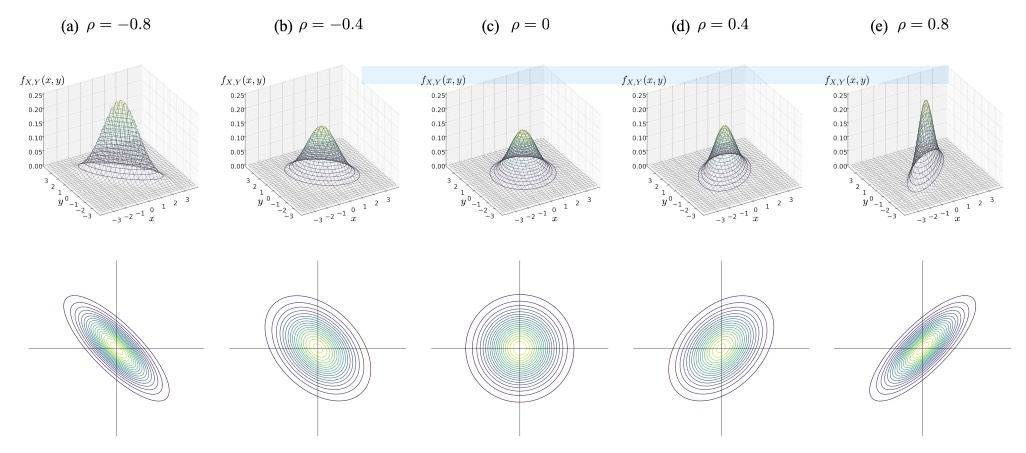
\includegraphics[width=.7\linewidth]{figures/prob4}
	\end{figure}
\end{enumerate}

\solution

See the code file.

\end{homeworkProblem}

\pagebreak

\begin{homeworkProblem}[3]

Let $X_1 \sim \operatorname{Expo}\left(\lambda_1\right), X_2 \sim \operatorname{Expo}\left(\lambda_2\right)$ and $X_3 \sim \operatorname{Expo}\left(\lambda_3\right)$ be independent.
\begin{enumerate}[(a)]
\item Find $E\left(X_1 \mid X_1>2024\right).$
\item Find $E\left(X_1 \mid X_1<1997\right).$
\item Find $E\left(X_1+X_2+X_3 \mid X_1>1997, X_2>2014, X_3>2025\right)$ in terms of $\lambda_1, \lambda_2, \lambda_3.$
\end{enumerate}

\solution

\begin{enumerate}[(a)]

\item According to the memoryless property of exponential distribution, we have $E(X_1-2023|X_1>2023)=E(X_1)$.
Thus we can obtain the conditional expectation as follows:
\begin{equation*}
	E(X_1|X_1>2024) = 2024 +E(X_1-2024|X_1>2024) =2024+E(X_1)=2024+\frac{1}{\lambda_1}.	
\end{equation*}

\item
\begin{equation*}
\begin{aligned}
	E(X_1|X_1<1997) 
	= ~& \frac{E(X_1) - E(X_1 | X_1 > 1997)P(X_1 > 1997)}{P(X_1 < 1997)} \\
	= ~& \frac{E(X_1) - (1997 + E(X_1))P(X_1 > 1997)}{P(X_1 < 1997)} \\
	= ~& E(X_1) - \frac{1997 \times P(X_1 > 1997)}{P(X_1 < 1997)} \\
	= ~& 1997 + E(X_1) - \frac{1997}{P(X_1 < 1997)} \\
	= ~& 1997 + \lambda_{1} - \frac{1997}{1 - e^{-\lambda_{1} 1997}} \\
\end{aligned}
\end{equation*}

\item Since $X_1,X_2,X_3$ are independent, we have
\begin{equation*}
\begin{aligned}
	~& E(X_1+X_2+X_3|X1>1997,X_2>2014,X_3>2025)\\
	= ~& E(X_1|X_1>1997,X_2>2014,X_3>2025)\\
	~& + E(X_2|X1>1997,X_2>2014,X_3>2025)\\
	~& + E(X_3|X_1>1997,X_2>2014,X_3>2025)\\
	= ~& E(X_1|X_1>1997)+E(X_2|X_2>2014)+E(X_3|X_3>2025)\\
	= ~& E(X_1-1997|X_1>1997)+E(X_2-2014|X_2>2014)+E(X_3-2025|X_3>2025)+6036\\
	= ~&  E(X_1)+E(X_2)+E(X_3)+6036\\
	= ~& \frac{1}{\lambda_1}+\frac{1}{\lambda_2}+\frac{1}{\lambda_3}+6036
\end{aligned}
\end{equation*}

\end{enumerate}

\end{homeworkProblem}

\pagebreak

\begin{homeworkProblem}[4]

Let $X$ and $Y$ be two continuous random variables with joint PDF
$$
f_{X, Y}(x, y)= \begin{cases}6 x y & \text { if } 0 \leq x \leq 1,0 \leq y \leq \sqrt{x}, \\ 0 & \text { otherwise. }\end{cases}
$$
\begin{enumerate}[(a)]
\item Find the marginal distributions of $X$ and $Y$. Are $X$ and $Y$ independent?
\item Find $E[X \mid Y=y]$ and $\operatorname{Var}[X \mid Y=y]$ for $0 \leq y \leq 1$.
\item Find $E[X \mid Y]$ and $\operatorname{Var}[X \mid Y]$.
\end{enumerate}

\solution

\begin{enumerate}[(a)]
	\item 
	The supports of $X$ and $Y$ are both $[0,1]$.
	In this way, we have
	\begin{equation*}
		\begin{aligned}
			f_{X}(x) 
			= ~& \int_{-\infty}^{\infty} f_{X, Y}(x, y) d y \\
			= ~& \int_{0}^{\sqrt{x}} 6xy dy \\
			= ~& 3 x y^{2} \Big|_{y = 0}^{y = \sqrt{x}} \\
			= ~& 3 x^{2},
		\end{aligned}
	\end{equation*}
	and 
	\begin{equation*}
		\begin{aligned}
			f_{Y}(y)
			= ~& \int_{-\infty}^{\infty} f_{X, Y}(x, y) d x \\
			= ~& \int_{y^{2}}^{1} 6 x y d x \\
			= ~& 3 y x^{2} \Big|_{x = y^{2}}^{x = 1} \\
			= ~& 3 y - 3y^{5}.
		\end{aligned}
	\end{equation*}
	Therefore, 
	\begin{equation*}	
		\begin{aligned}
			f_{X}(x) 
			= ~& \begin{cases} 
				3 x^{2}  & \text{if} \ 0 \le x \le 1, \\
				0     & \text{otherwise}.
			\end{cases} \\
			f_{Y}(y) 
			= ~& \begin{cases} 
				3 y - 3y^{5}  & \text{if} \ 0 \le y \le 1, \\
				0     & \text{otherwise}.
			\end{cases}
		\end{aligned}			
	\end{equation*}
	Since $f_{X, Y}(x, y) \ne f_{X}(x)f_{Y}(y)$, $X$ and $Y$ are not independent.
	
	\item
	Since
	\begin{equation*}
		E[X | Y=y]
		= \int_{-\infty}^{\infty} x f_{X | Y}(x | y) d x,
	\end{equation*}
	to calculate $E[X | Y=y]$, we need to first calculate $f_{X | Y}(x | y) $.
	
	If $y^2 \le x \le 1$, 
	\begin{equation*}
		f_{X | Y}(x | y)
		= \frac{f_{X, Y}(x, y)}{f_{Y}(y)}
		= \frac{2x}{1-y^{4}}.
	\end{equation*}
	In this way, 
	\begin{equation*}
		f_{X | Y}(x | y)
		= \begin{cases} 
			\frac{2x}{1-y^{4}} & \text{if} \ y^{2} \le x \le 1, \\
			0     & \text{otherwise}.
		\end{cases}
	\end{equation*}
	Therefore, 
	\begin{equation*}
		\begin{aligned}
			E[X | Y=y]
			= ~& \int_{-\infty}^{\infty} x f_{X | Y}(x | y) d x \\
			= ~& \int_{y^{2}}^{1} x \frac{2x}{1-y^{4}}  d x \\
			= ~& \frac{2}{3(1-y^{4})}x^{3} \Big|_{x = y^{2}}^{x = 1}  \\
			= ~& \frac{2(1 - y^{6})}{3(1-y^4)} \\
			= ~& \frac{2}{3}\cdot\frac{1+y^{2}+y^{4}}{1+y^{2}}
		\end{aligned}
	\end{equation*}

	Since
	\begin{equation*}
		\text{Var}[X|Y=y] 
		= E[X^{2} | Y=y] - (E[X | Y=y])^{2},
	\end{equation*}
	to calculate $\text{Var}[X|Y=y]$, we need to first calculate $E[X^{2} | Y=y] $.
	
	Since
	\begin{equation*}
		\begin{aligned}
			E[X^{2} | Y=y]
			= ~& \int_{-\infty}^{\infty} x^{2} f_{X | Y}(x | y) d x \\
			= ~& \int_{y^{2}}^{1} x^{2} \frac{2x}{1-y^{4}}  d x \\
			= ~& \frac{1}{2(1-y^{4})}x^{4} \Big|_{x = y^{2}}^{x = 1}  \\
			= ~& \frac{1 - y^{8}}{2(1-y^{4})} \\
			= ~& \frac{1 + y^{4}}{2},
		\end{aligned}
	\end{equation*}
	we have, 
	\begin{equation*}
		\begin{aligned}
			\text{Var}[X|Y=y] 
			= ~& E[X^{2} | Y=y] - (E[X | Y=y])^{2} \\
			= ~& \frac{1 + y^{4}}{2} - \left(\frac{2(1 - y^6)}{3(1-y^4)}\right)^2 \\
			= ~& \frac{1+y^{4}}{2}-\frac{4}{9}\cdot\frac{(1+y^{2}+y^{4})^{2}}{(1+y^{2})^{2}} 
		\end{aligned}
	\end{equation*}
	\item
	According to the result in question(b), we have
	\begin{equation*}
	\begin{aligned}
		& E[X|Y] = \frac{2}{3}\cdot\frac{1+Y^{2}+Y^{4}}{1+Y^{2}}, \\
		& \operatorname{Var}[X|Y] = \frac{1+Y^{4}}{2} - \frac{4}{9}\cdot\frac{(1+Y^{2}+Y^{4})^{2}}{(1+Y^{2})^{2}}.
	\end{aligned}
	\end{equation*}

\end{enumerate}

	
\end{homeworkProblem}

\pagebreak

\begin{homeworkProblem}[5]

Let $X$ be a discrete r.v. whose distinct possible values are $x_0, x_1, \ldots$, and let $p_k = P (X = x_k)$.
The entropy of $X$ is $H(X) = \sum_{k=0}^{\infty} p_k \log_2 (1 / p_k )$.

\begin{enumerate}[(a)]
	\item Find $H(X)$ for $X \sim \operatorname{Geom}(p)$.
	\item Let $X$ and $Y$ be i.i.d. discrete r.v.s. Show that $P(X = Y) \geq 2^{-H(X)}$. Hint: Jensen's Inequality.
\end{enumerate}

\solution

\begin{enumerate}[(a)]

\item The PMF of $X$ is $P(X=k) = p(1-p)^k$ since there is $X \sim \operatorname{Geom}(p)$.
Thus we have 
\begin{equation*}
\begin{aligned}
	H(X)
	&= - \sum_{k=0}^{\infty} p(1-p)^k \log_2 \Big( p(1-p)^k \Big) \\
	&= -p\sum_{k=0}^{\infty} k(1-p)^k \log_2 (1-p) - p \log_2 p \sum_{k=0}^{\infty} (1-p)^k \\
	&= -\log_2 {p} - \frac{1-p}{p} \log_2 (1-p)
\end{aligned}
\end{equation*}

\item Since $X$ and $Y$ are i.i.d random variables, via LOTP, we have
\begin{equation*}
\begin{aligned}
	P(X=Y)
	&= \sum_{k=0}^{\infty}P(X=Y|Y=k)\cdotp P(Y=k)\\
	&= \sum_{k=0}^{\infty}P(X=k)\cdotp P(Y=k)
	= \sum_{k=0}^{\infty}p_k^2
\end{aligned}
\end{equation*}

Denote $Z$ as a new discrete random variable such that $P(Z=p_k) = p_k$, then we have:
\begin{equation*}
	E(Z) = \sum_{k=0}^{\infty} p_k \times p_k = P(X=Y) 
\end{equation*}

Since $\log(\cdot)$ is a convex function, according to Jensen's inequality, we have $E(\log(Z)) \leq \log(E(Z))$, thus there is 
\begin{equation*}
\begin{aligned}
	& \sum p_k \log_2 p_k \leq \log_2\sum p_k^2 \\
	\Leftrightarrow & -H(X) \leq \log_2 P(X=Y) \\
	\Leftrightarrow & P(X=Y) \geq 2^{-H(X)}.
\end{aligned}
\end{equation*}
    
\end{enumerate}

\end{homeworkProblem}

\pagebreak

\begin{homeworkProblem}[6]

Instead of predicting a single value for the parameter, we give an interval that is likely to contain the parameter:
A $1-\delta$ confidence interval for a parameter $p$ is an interval $[\hat{p}-\epsilon, \hat{p}+\epsilon]$ such that $P(p \in[\hat{p}-\epsilon, \hat{p}+\epsilon]) \geq 1-\delta$.
Now we toss a coin with probability $p$ landing heads and probability $1-p$ landing tails.
The parameter $p$ is unknown and we need to estimate its value from experiment results.
We toss such coin $N$ times.
Let $X_i = 1$ if the $i$th result is head, otherwise $0$.
We estimate $p$ by using
\begin{equation*}
	\hat{p} = \frac{X_1+\ldots+X_N}{N}.	
\end{equation*}

Find the $1 - \delta$ confidence interval for $p,$ then discuss the impacts of $\delta$ and $N$.

\begin{enumerate}[(a)]
	\item Method 1: Adopt Chebyshev inequality to find the $1-\delta$ confidence interval for $p$, then discuss the impacts of $\delta$ and $N$.
	\item Method 2: Adopt Hoeffding bound to find the $1-\delta$ confidence interval for $p$, then discuss the impacts of $\delta$ and $N$.
	\item Discuss the pros and cons of the above two methods.
\end{enumerate}

\solution

Since $X_{i} \sim \operatorname{Bern}(p), X_{i} \in \{0, 1 \}$, we have $\mathbb{E}[X_{i}] = p$ and $\mathbb{V}[X_{i}] = p(1 - p)$.
Therefore, we have
\begin{equation*}
	\mathbb{E}[\hat{p}] = p, \mathbb{V}[\hat{p}] = \frac{p(1-p)}{N}.
\end{equation*}
Besides, we know that
\begin{equation*}
	P(p\in[\hat{p}-\varepsilon,\hat{p}+\varepsilon])\geq 1 - \delta \Leftrightarrow P(|\hat{p}-p|\geq\varepsilon) \leq \delta.
\end{equation*}

\begin{enumerate}[(a)]
    \item 
    Applying Chebyshev's inequality on random variable $\hat{p}$, we have 
    \begin{equation*}
    	P(|\hat{p} - p| \geq \epsilon) \leq \frac{p(1 - p)}{N \epsilon^2}
    	\Rightarrow \delta = \frac{p(1 - p)}{N \epsilon^2}, \epsilon = \sqrt{ \frac{p(1 - p)}{N \delta} }
    \end{equation*}
    Therefore, we know that $ \delta $ negatively correlates with $\epsilon$, i.e., given a fixed number of samples $N$, there is natural trade-off between accuracy and confidence.
    Besides, 1) Fix the confidence interval parametrized by $\delta,$ reducing the estimation error $\epsilon$ requires increasing the number of samples $N$. 
    2) Fix the estimation error $\epsilon,$ narrowing the confidence interval requires increasing the number of samples $N$.
    That is, the impacts of $N$ is on both the ``estimation accuracy'' and ``estimation confidence''.
    
    \item 
    Applying Hoeffding's inequality on random variable $\hat{p}$, we have
    \begin{equation*}
    	P(|\hat{p} - p| \geq \epsilon) \leq 2 e^{- 2 N \epsilon^{2}}
    	\Rightarrow \delta = 2 e^{- 2 N \epsilon^{2}}, \epsilon = \sqrt{ \frac{\ln (2 / \delta)}{2N} }
    \end{equation*}
    The effects of $\delta$ and $N$ are similarly discussed as in $(a)$.
    
    \item 
    Chebyshev's inequality (see Cantelli's inequality for the one-side improvement):
    \begin{itemize}
        \item Pros: 1) sharp bound and cannot be improved in general (given no extra assumption). 2) can be improved with extra distributional information on polynomial moments.
        \item Cons: 1) requires the existence of moments until the second order. 2) quadratic convergence rate.
    \end{itemize}

    Hoeffding's inequality (see Theorem 2.8 and 2.9 of paper ``old and new concentration inequalities'' for the one-side improvement):
    \begin{itemize}
        \item Pros: 1) exponential convergence rate. 2) does not require assumption on moments.
        \item Cons: 1) works only for sub-Gaussian (e.g., bounded random variables). 2) in general not sharp when the variance is small (e.g., see popoviciu's inequality on variances and Bernstein's inequality).
    \end{itemize}

\end{enumerate}
\end{homeworkProblem}

\pagebreak

\begin{homeworkProblem}[7]

We consider the progressive Monty Hall problem.
This time we assume there are $n$ identical doors, where $n$ is an integer satisfying $n \geq 3$.
One door conceals a car, the other $n-1$ doors conceal goats.
You choose one of the doors at random but do not open it.
Monty then opens a door he knows to conceal a goat, always choosing randomly among the available doors.
At this point he gives you the option either of sticking with your original door or switching to one of the remaining doors.
You make your decision.
Monty now eliminates another goat-concealing door (at random) and once more gives you the choice either of sticking or switching.
This process continues until only two doors remain in play.
What strategy should you follow to maximize your chances of winning?
We consider three strategies:
(1) Select a door at random and stick with it throughout.
(2) Select a door at random, then switch doors at every opportunity, choosing your door randomly at each step. 
(3) Select a door at random, stick with your first choice until only two doors remain, and then switch.
{\bf When $n = 4$ and $n = 100$, please use simulation to compare such three strategies.}

\solution

See the code file.

\end{homeworkProblem}

\pagebreak

\end{document}
